\chapter{Organización de la información}

\section{Diseño}
La información se organiza en una estructura  jerárquica. La estructura se compone de las entidades presentes en la ontología, de manera que las entidades más relevantes se encuentran en el primer nivel de jerarquía, y a medida que se desciende por los niveles la importancia de las entidades disminuye.

Para alcanzar esta estructura, se crearon una serie de módulos que transforman la entrada hasta alcanzar un árbol con toda la información que posee la ontología. El primer módulo recibe la entrada y crea una representación interna de la ontología, luego esta representación es enviada a otros dos módulos: uno se encarga de extraer las entidades más relevantes; el otro, con la representación interna de la ontología y las entidades más relevantes, se encarga de generar un árbol de entidades. Para finalizar, un último módulo se asegura de agregar aquellas entidades que no han sido utilizadas en ninguna rama del árbol, creando una rama especial del árbol en el que se insertan las entidades que no han sido relacionadas con las demás.

En la figura \ref{fig:modulos_organizador_inf} se muestran los módulos que transforman la entrada en la jerarquía esperada.

\begin{figure}[H]
    \centering
    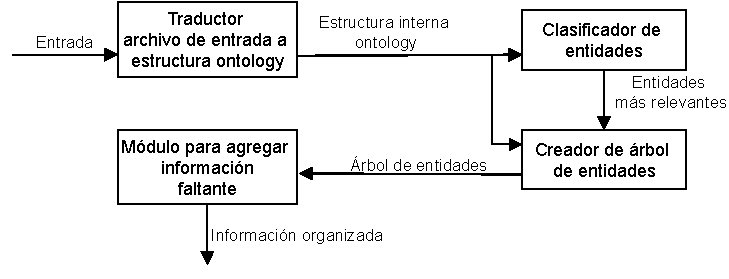
\includegraphics[width=12cm, height=6cm]{img/organizacion_informacion/modulos_organizador_de_informacion.pdf}
    \caption{Módulos que componen el organizador de información}
    \label{fig:modulos_organizador_inf}
\end{figure}

\subsection{Representación interna de la ontología}

El módulo que crea la representación interna de la ontología se encarga de cargar toda la información de la ontología para poder se accedida con mayor facilidad. Como algunos datos son accedidos a través de un razonador o importados de otras ontologías, se optó por cargar toda esta información una única vez para reducir el tiempo de respuesta cuando se requieren esos datos.

\subsection{Clasificación de las entidades más relevantes}
Una vez creada la representación de la ontología, el segundo módulo debe clasificar las entidades y extraer las más relevantes. A continuación se explicará cómo son extraídas estas entidades.

\subsubsection{Criterio de clasificación}
Para este trabajo, asumimos que los grafos subyacentes a las ontologías usadas en la web semántica están caracterizados por ser grafos libres de escala ~\cite{zhang2008scale}. Considerando esta hipótesis, esperamos que la naturaleza de las relaciones brinden información suficiente para discriminar entre el contenido principal y el menos relevante.

El criterio principal para establecer una clasificación sobre las clases de una ontología, y que tal clasificación sirva para seleccionar las clases más relevantes para la verbalización de la ontología, se basa en cuánta información posee una clase respecto al resto de las clases en la ontología. En este trabajo se considera la mayor cantidad de información, a aquellas clases que están presentes en la mayor cantidad de dominios de \emph{ObjectProperties}. Esto permite obtener las clases que tengan mayor cantidad de conexiones con otras clases, y que a su vez sean el núcleo de la relación. Teniendo en cuenta a las clases mejor clasificadas, se puede centrar lo que se dice en el texto alrededor de estas clases.

Visualizando la ontología como un grafo, se puede considerar el grado del nodo como valor para clasificar las clases, pero teniendo en cuenta para el cálculo del grado únicamente los arcos que  
unen a los nodos a través de la relación \emph{rdf:domain}.

Algunas ventajas de este enfoque son:
\begin{itemize}
    \item Sencillez de implementación. Únicamente se debe recorrer el grafo calculando el valor de cada nodo. El recorrido del grafo tiene a lo sumo una complejidad polinomial.
    \item No se requiere agregar información extra al dominio.
    \item No es necesario utilizar sobre la ontología un razonador que requiera una complejidad computacional que sea intratable. La única observación es que hay que inferir el dominio y rango de las \emph{ObjectProperties}. Sin embargo, la inferencia de dominio y rango se realiza teniendo en cuenta la jerarquía de \emph{ObjectProperties}, sin necesidad de inferir clases equivalentes o disjuntas.
\end{itemize}

La eficacia de este enfoque depende fuertemente de que las \emph{ObjectProperties} más importantes tengan el dominio explícito.


\subsubsection{Seleccionando las principales clases}
\label{sec:select_class}
Una vez calculado el valor de cada clase, se pueden seleccionar las clases que superen cierto umbral para remover las menos importantes. En este trabajo, se recorren todas las clases y se seleccionan las que superen el valor promedio entre cantidad de propiedades y cantidad de clases.

Además, se estableció un factor de reducción del umbral, para el caso en el que no exista ninguna clase que supere el umbral seleccionado. Este factor reduce el umbral en 10\%, y se recorren todas las clases nuevamente. Iterativamente, el umbral es reducido hasta encontrar alguna clase que lo supere, o hasta llegar a cero.

Cuando se seleccionan las clases que van a representar los temas principales, puede ocurrir que se elijan clases de una misma rama en la jerarquía de clases. Esto hace que se pierda algo de semántica, pues se incluyen clases en el mismo nivel, siendo que algunas son más específicas y pueden ser alcanzadas desde sus ancestros. Para evitar este problema, se optó por eliminar las subclases que sean seleccionadas en un principio, y que tengan a una clase ancestro dentro de los temas principales.

En la figura \ref{fig:diagrama_secuencia_getMainContent} se presenta un pseudocódigo del algoritmo usado para seleccionar las clases principales.

\begin{figure}[H]
    \centering
    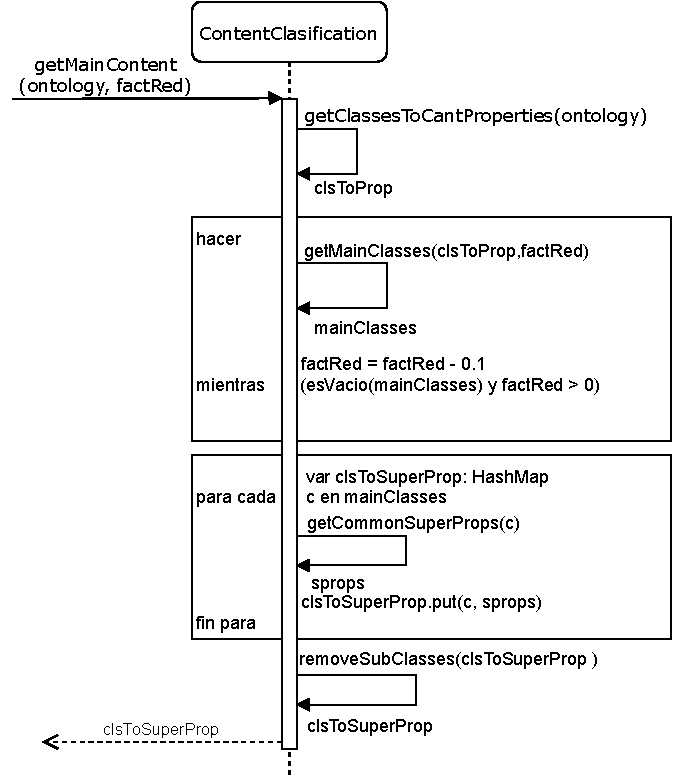
\includegraphics[width=8cm, height=7cm]{img/organizacion_informacion/secuencia_getMainContent.pdf}
    \caption{Diagrama de secuencia para seleccionar las clases principales}
    \label{fig:diagrama_secuencia_getMainContent}
\end{figure}


\subsection{Agrupando la información de las clases elegidas}
\label{sec:agrupando_info}
Una vez elegidas las clases que serán los temas principales del texto, se procede a crear el árbol completo, con toda la información relacionada a estas clases. Para esto se creó un tercer módulo, que agrupa la información de cada entidad en grupos generales, que abarquen con el mayor nivel de abstracción  posible su información. Para esto, para cada clase, se busca reemplazar las propiedades donde participan como dominio, por propiedades en común de más alto nivel en la jerarquía de \emph{ObjectProperties}. Por ejemplo, en la ontología de las pizzas, para la clase \emph{pizza} existen dos propiedades: \emph{tieneCobertura} y \emph{tieneBase}. Como estas dos propiedades tienen a su vez una \emph{superproperty} en común llamada \emph{tieneIngrediente}, se agrupa toda la información que pueda ser alcanzada por las \emph{subproperties} en un único grupo representado por \emph{tieneIngrediente}. 

Además de la información que puede ser alcanzada desde las \emph{ObjectProperties}, la información que poseen las subclases y los individuos también es de suficiente valor para ser agrupada. En este sentido, las unidades de información representadas por las subclases y los individuos de cada clase elegida como tema relevante, son también incluidas en un grupo. En este caso estamos haciendo uso de las relaciones \emph{owl:subClassOf} y \emph{owl:NamedIndividual}.

En la figura \ref{fig:diagrama_secuencia_contentGrouping} se muestra un pseudocódigo del algoritmo usado para agrupar la información de las clases.

Con toda esta información, se crea un primer nivel de grupos que abarcan lo más general posible todos los temas a ser tratados en un texto. Como ejemplo, el primer nivel de la ontología de las pizzas quedaría como en la figura \ref{fig:macro_planning_pizza}.
\begin{figure}[H]
%no borrar el % de dirtree porque es necesario.
\dirtree{%
.1 pizza.
.2 tieneIngrediente.
.2 pizzaConCarne.
.2 pizzaConNombre.
.2 $...$ las restantes subclases de pizza.
}
\caption{Organización del contenido de la ontología \emph{pizza}.}
\label{fig:macro_planning_pizza}
\end{figure}

\begin{figure}[H]
    \centering
    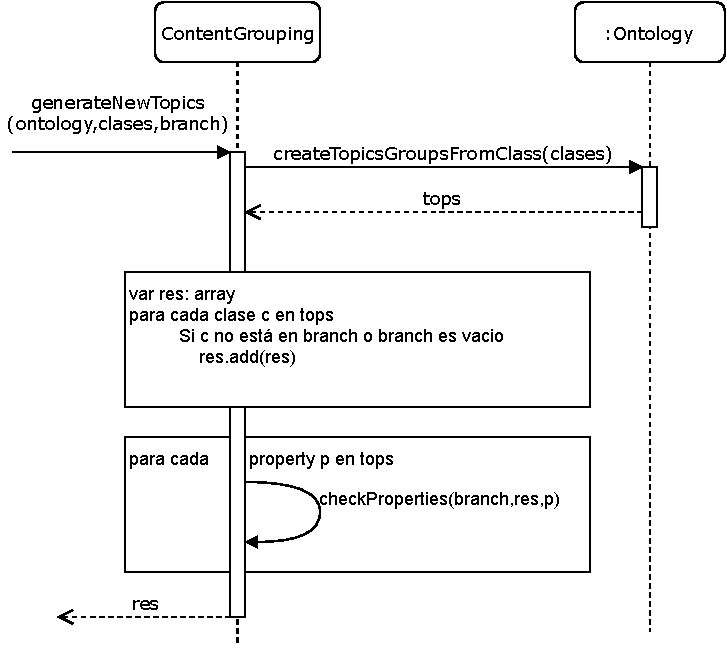
\includegraphics[width=8cm, height=7cm]{img/organizacion_informacion/secuencia_contentGrouping.pdf}
    \caption{Diagrama de secuencia para agrupar la información de las clases}
    \label{fig:diagrama_secuencia_contentGrouping}
\end{figure}


\subsubsection{Recorriendo la ontología}
Luego de obtener el primer grupo de información, queda pendiente tratar el segundo problema nombrado en \ref{sec:problema_coherencia-texto}: recorrer la ontología obteniendo y agrupando la información relacionada a los temas elegidos. 

El objetivo es establecer una jerarquía de grupos de información, comenzando desde los elementos del primer grupo, que abarcan la información más general, e ir creando nuevos grupos con información más específica. De esta manera, se garantiza que entre los elementos pertenecientes a una rama haya una relación semántica.

Partiendo desde el primer nivel (como los de la figura \ref{fig:macro_planning_pizza}), se aplica el mismo algoritmo usado en \ref{sec:agrupando_info} para obtener el contenido principal, pero esta vez sobre cada elemento del primer nivel. Como ahora es posible que un elemento sea una \emph{ObjectProperty}, para continuar el recorrido de la ontología se buscan sus subproperties, para luego continuar obteniendo información de ellas. Las subproperties elegidas deben contener en su dominio, a la clase que haya sido elegida como tópico para ese grupo de información que se está creando. La búsqueda de subproperties debe ser exhaustiva, pues si no se encuentran subproperties que tengan en su dominio a la clase tópico, debe continuar la búsqueda bajando en la jerarquía de propiedades hasta hallar alguna, ya que es el proceso inverso a la búsqueda de superproperties en común usadas para agrupar la información de manera más general. Si no hay subproperties, entonces la nueva información para agregar en el texto se basa en el rango de la \emph{ObjectProperty} inicial. En este último caso, empleamos la relación \emph{rdf:Range}.

Continuando con el ejemplo de la ontología de la pizza, expandimos la figura \ref{fig:macro_planning_pizza} con el siguiente nivel de información, en la figura \ref{fig:macro_planning_pizza_n2}. 
\begin{figure}[H]
%no borrar el % de dirtree porque es necesario.
\dirtree{%
.1 pizza.
.2 tieneIngrediente.
.3 tieneBase.
.3 tieneCobertura.
.2 pizzaConCarne.
.2 pizzaConNombre.
.3 Margherita.
.3 Napoletana.
.3 $...$ las restantes subclases de pizzaConNombre.
.2 $...$ las restantes subclases de pizza, con sus respectivas subclases.
}
\caption{Organización del contenido de nivel dos de la ontología \emph{pizza}.}
\label{fig:macro_planning_pizza_n2}
\end{figure}

Se puede ver que las subproperties \emph{tieneBase} y \emph{tieneCobertura} tienen en su dominio a \emph{pizza}, la clase más cercana recorriendo sus ancestros. Si existiera por ejemplo, \emph{tieneCondimento} como una tercer subproperty de \emph{tieneIngrediente}, cuyo dominio no tuviera \emph{pizza}, entonces no sería listada dentro del grupo \emph{tieneIngredientes} en la rama de \emph{pizza}. Sin embargo, deben explorarse las subproperties de \emph{tieneCondimento}, por el caso de que tenga alguna subproperty que tuviera como dominio a \emph{pizza}. Por ejemplo, supongamos que \emph{tieneCondimento} tiene como subproperty a \emph{tieneOrégano} con diminio \emph{pizza}, en ese caso se habilita a \emph{tieneCondimento} para ser insertado en el grupo junto a  \emph{tieneCobertura} y \emph{tieneBase}.  

De esta manera, el mismo algoritmo se aplica recursivamente para cada elemento de cada nivel. El algoritmo se detiene cuando no encuentra más subclases ni propiedades para cada clase del último nivel.

\subsection{Agregando información marginada}
Con el recorrido de la ontología para formar los grupos de información, existe la posibilidad de que hayan clases que no sean parte de un grupo. Es el caso, por ejemplo, de la clase \emph{Comida}, y sus subclases \emph{Helado} y \emph{Condimento}, en la ontología \emph{pizza}. Para no dejar información del dominio excluida en el árbol, se ejecuta un cuarto módulo, que crea un nuevo grupo menos importante, y se agregan todas las clases que habían quedado marginadas. El proceso de creación de subgrupos para este nuevo grupo es idéntico al explicado en las sección anterior.

Continuando con el ejemplo de la pizza, el resultado de agregar la  información marginada se muestra en la figura \ref{fig:macro_planning_pizza_marg}

\begin{figure}[H]
%no borrar el % de dirtree porque es necesario.
\dirtree{%
.1 pizza.
.2 ....
.1 comida.
.2 condimento.
.2 helado.
}
\caption{Grupos de la ontología \emph{pizza} con información marginada.}
\label{fig:macro_planning_pizza_marg}
\end{figure}

\subsection{Diagrama de clases}
En la figura \ref{fig:diagrama_clases_organizador} se muestra el diagrama de clases correspondiente al organizador de información. El primer módulo tiene asociado las clases \emph{Ontology} y \emph{OWLIntClass}. El segundo módulo está representado por la clases \emph{ContentClasification}; y el tercer y cuarto módulo están asociados a la clase \emph{ContentGrouping}.

\begin{figure}[H]
    \centering
    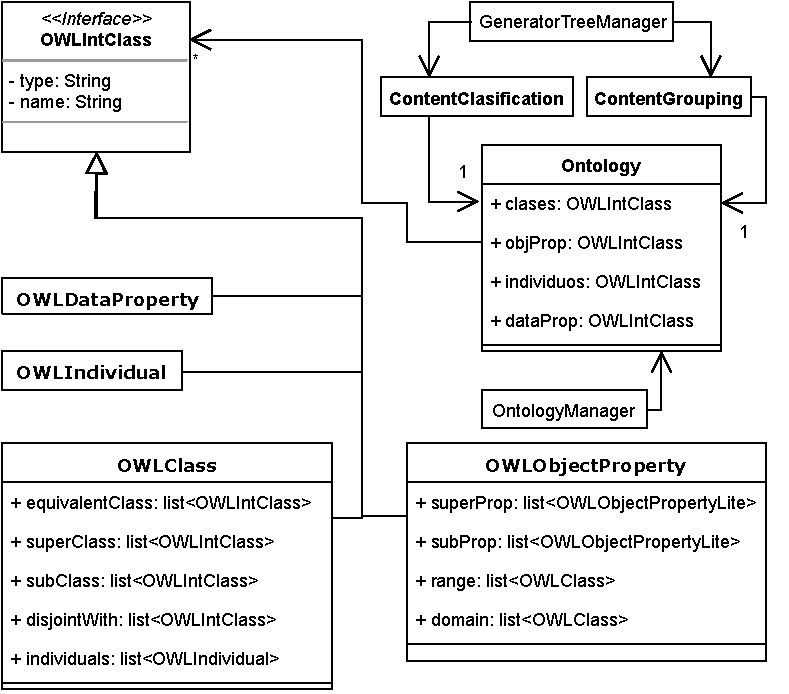
\includegraphics[width=10cm]{img/organizacion_informacion/clases_organizador_informacion.pdf}
    \caption{Diagrama de clases del organizador de información}
    \label{fig:diagrama_clases_organizador}
\end{figure}

\section{Implementación}
\subsection{blabla}

\section{Casos de estudio}
En esta sección se presentan tres casos de estudio que muestran el comportamiento de la aplicación ante tres entradas diferentes, abarcando distintos aspectos de la solución propuesta.

Al momento de realizar este trabajo no se reconoce ninguna aplicación que aborde el problema de organización de la información en una ontología, por lo que se expondrán tres casos de estudio sin la posibilidad de compararlos con otros resultados.

\subsection{Organización de Ontología Pizza}
Según la descripción de la ontología, este dominio representa las pizzas y sus coberturas, por lo que esperamos que las entidades que representen a las pizzas, a las coberturas y la información complementaria tiendan a agruparse en los niveles más altos de la jerarquía, mientras que en los niveles más bajas esperamos encontrar las clases más específicas y que tienen menor impacto sobre el entendimiento del dominio.

En la figura \ref{fig:caso_estudio_pizza} se puede ver el resultado de aplicar el algoritmo teniendo como entrada la ontología pizza. 

Los nombres de las entidades fueron traducidos al español, para poder generar las sentencias en lenguaje español en el siguiente capítulo, pero el idioma no afecta los resultados del algoritmo propuesto.

\begin{figure}
\begin{multicols}{2}
\begin{figure}[H]
\dirtree{%
.1 Pizza.
.2 Pizza con nombre.
.3 Margherita.
.3 Frutti di mare.
.3 Giardiniera.
.3 ....
.3 Napoletana.
.2 Pizza con carne.
.2 Pizza picante.
.2 ....
.2 Pizza vegetariana.
.2 Ingredientes.
.3 Coberturas.
.4 Cobertura de pizza.
.5 Cobertura de verduras.
.6 Cobertura de pimiento.
.6 ....
.6 Cobertura de langostinos.
.3 Bases.
.4 Base de pizza.
.5 Base gruesa.
.5 Base delgada y crujiente.
.5 Condimentoes.
.6 Sales.
.7 Sal.
}
\end{figure}

\begin{figure}[H]
\dirtree{%
.1 Otras secciones.
.2 Domain concept.
.3 Comida.
.4 Helado.
.4 Ingrediente.
.3 Pais.
.4 America.
.4 England.
.4 Italy.
.4 France.
.4 Germany.
.2 Value partition.
.3 Picante.
.4 Poco picante.
.4 Algo picante.
.4 Muy picante.
}
\end{figure}

\end{multicols}
\caption{Resultado del organizador de información con la ontología Pizza.}
\label{fig:caso_estudio_pizza}
\end{figure}

La ontología pizza cuenta con 100 clases y 8 propiedades. De las 8 propiedades, 5 fueron usadas  para clasificar las 100 clases (de las 8, 3 eran inversas a otras 3 por lo que no agregaban información nueva). El promedio de información obtenido fue 1.25, siendo la clase Pizza la única en superar este valor, lo que concuerda con el resultado esperado.

Como se puede observar en la figura \ref{fig:caso_estudio_pizza}, en la primer columna se encuentran los tópicos principales reconocidos por el algoritmo, y en la segunda columna se encuentran los tópicos agregados con el módulo para agregar información marginada.

En la jerarquía de los tópicos principales, se puede ver como toda la información se agrupa como hijas de la entidad Pizza, describiendo los tipos de pizzas y sus ingredientes. Inmediato a los ingredientes lista las coberturas, y reconoce a las bases de pizza a la misma altura que las coberturas, asignándoles la misma importancia.

En la jerarquía de \emph{otras secciones}, se aprecian las demás entidades que aportan información secundaria a la descripción del dominio, que no está directamente relacionada con el dominio de las pizzas, como son los países, los tipos de picante y otras comidas.

Respecto al resultado esperado, la organización de la información es satisfactoria, ya que se asimila a la propia descripción del dominio. 

\subsection{Organización de Ontología Wine}
Esta ontología tiene como objetivo describir un dominio de vinos y comidas\footnote{\url{https://protege.stanford.edu/publications/ontology_development/ontology101-noy-mcguinness.html}}, por lo que esperamos que las entidades que se consideren más relevantes sean aquellas afines a los vinos y comidas.

En la figura \ref{fig:caso_estudio_wine} se puede ver el resultado de aplicar el algoritmo teniendo como entrada la ontología Wine.

\begin{figure}
\begin{multicols}{2}
{\small
\begin{figure}[H]
\dirtree{%
.1 Wine.
.2 Italian wine.
.3 Chianti.
.4 Chianti classico.
.2 $...$ \emph{(otras subclases de Wine)}.
.2 Wines descriptor.
.3 Sugar.
.4 Wine sugar.
.5 Dry.
.5 Off dry.
.5 Sweet.
.3 Colors.
.4 Wine color.
.5 White.
.5 Rose.
.5 Red.
.3 Flavors.
.4 Wine flavor.
.5 Moderate.
.5 Strong.
.5 Delicate.
.3 Bodies.
.4 Wine body.
.5 Medium.
.5 Full.
.5 Light.
.2 From grapes.
.3 Wine grape.
.4 Chenin blanc grape.
.4 $...$ \emph{(otras subclases de Wine grape)}.
}
\end{figure}}  

\begin{figure}[H]
\dirtree{%
.1 Otras secciones.
.1 Region.
.2 Central texas region.
.2 $...$ \emph{(otras subclases de Region)}.
.1 Vintage year.
.2 Year1998.
.1 Wine descriptor.
.2 Wine taste.
.1 Non consumable thing.
.1 Vintage.
.2 Vintage years.
.1 Fruit.
.1 Winery.
.2 Chateau de meursault.
.2 $...$ \emph{(otras subclases de Winery)}.
.1 Consumable thing.
.2 Meal.
.3 Courses.
.4 Meal course.
.5 Cheese nuts dessert course.
.5 $...$ \emph{(otras subclases de Meal course)}.
.5 Foods.
.6 Edible thing.
.7 Fowl.
.8 $...$.
.7 Dessert.
.8 $...$.
.7 Meat.
.8 $...$.
.7 Seafood.
.8 $...$.
.7 Sweet fruit.
.8 Grape.
.8 $...$.
.7 Pasta.
.8 $...$.
.7 Non sweet fruit.
.5 Drinks.
.6 Potable liquid.
.7 Juice.
.7 Wine.
.8 Wines descriptor.
.8 From fruits.
}
\end{figure}

\end{multicols}
\caption{Resultado del organizador de información con la ontología Wine.}
\label{fig:caso_estudio_wine}
\end{figure}


La ontología Wine cuenta con 138 clases y 16 propiedades. De las 16 propiedades, 12 fueron usadas para verificar qué clases superan el umbral promedio para ser seleccionadas como las principales. El promedio fue de 2.5 y la única clase que lo superó fue Wine, lo que cumple parcialmente el resultado esperado, ya que parte del objetivo de la ontología es describir el dominio de los \emph{Wines}. Respecto a la sección que describe las comidas, quedó desplazada a \emph{otras secciones}, siendo un resultado no esperado según el objetivo de la ontología. Sin embargo, analizando manualmente la ontología, se puede apreciar que el porcentaje de  información que describe a las comidas es significativamente menor en relación a la información referida a los vinos, factor por el cual resulta aceptable que no aparezcan como sección principal.

\subsection{Organización de Ontología SNOMED-CT}

\section{Conclusiones}